\documentclass{article}
\usepackage[utf8]{inputenc}
\usepackage{geometry}
\geometry{a4paper,left=42mm,top=28mm,right=42mm,down=28mm}
\usepackage{multicol}
\usepackage{blindtext}
\usepackage{graphicx}
\usepackage{caption}
\usepackage{tabularx}
\usepackage[english,russian]{babel}
\usepackage{fancyhdr}
\usepackage{anyfontsize}
\usepackage{multirow}

\pagestyle{fancy}
\fancyhf{}
\renewcommand{\headrulewidth}{0pt}
\lfoot{\thepage}

\DeclareCaptionLabelFormat{ris}{\textbf{Рис}. #2.}
\setcounter{page}{46}
\setcounter{figure}{5}


\begin{document}

\begin{figure}[ht]
   \minipage{0.35\textwidth}
  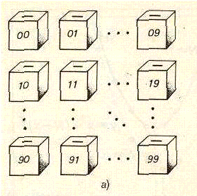
\includegraphics[width=\linewidth]{Image_1.png}
  \textbf{Рис}. 5.
\endminipage\hfill
\minipage{0.65\textwidth}
  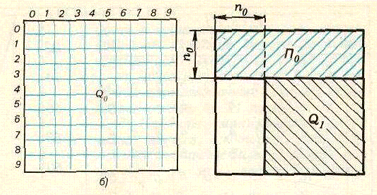
\includegraphics[width=\linewidth]{Image_2.png}
  \captionsetup{labelformat=ris,labelsep=quad}
  \caption{}
\endminipage\hfill
\end{figure}
\begin{multicols}{2}
\noindent
ток,\hfillа\hfillименно\hfill$n_0$,\hfillзакрашено в нуле-\\*
вой\hfillстрочке;\hfillможно\hfillсчитать,\hfillчто\hfillэто\\*
первые\hfill$n_0$\hfillклеток\hfillстрочки.\hfillРассмот-\\*
рим\hfillтеперь\hfillквадрат\hfill$Q_r$,\hfillполучающий-\\*
ся\hfillиз\hfill$Q_0$\hfillвычеркиванием\hfillпервых\hfill$n_0$\\*
строчек\hfillи\hfillпервых\hfill$n_0$\hfillстолбцов\hfill(рис. 6).\\*
Покажем,\hfillчто\hfillвсе\hfillклетки\hfill$Q_1$\hfillдолжны\\*
быть\hfillзакрашены.\hfillДля\hfillэтого\hfillвозьмем\\*
ящики\hfillс\hfillномером\hfill$xy$,\hfillгде\hfill$x\geq n_0$,\\*
$y\geq n_0$.\hfillВ\hfillнего\hfillобязательно\hfillпопадает\\*
билет\hfill$0xy$:\hfillего\hfillнельзя\hfillположить\\*
в\hfillящики\hfill$0x$\hfillи\hfill$0y$,\hfillтак\hfillкак\hfillсоответст-\\*
вующие\hfillклетки\hfillне\hfillзакрашены.\\*
Значит,\hfillклетка\hfillс\hfillномером\hfill$xy$\hfillдолжна\\*
быть\hfillзакрашена\hfillдля\hfillвсех\hfill$x\geq n_0$,\\*
$y\geq n_0$.

Посчитаем,\hfillсколько\hfillже\hfillвсего\hfillкле-\\*
ток\hfillзакрашено\hfillв\hfillнашем\hfillквадрате\hfill$Q_0$.\\*
В\hfillкаждой\hfillстрочке\hfillпрямоугольника\\*
$П_0$\hfill(см. рис. 6)\hfillзакрашено\hfillпо\hfillкрай-\\*
ней\hfillмере\hfill$n_0$\hfillклеток.\hfillВ\hfill$Q_1$\hfillзакрашены\\*
все\hfill$(10-n_0)^2$\hfillклеток.\hfillТаким\hfillобразом,\\*
в\hfill$Q_0$\hfillзакрашено\hfillпо\hfillкрайней\hfillмере\\*
$n_0^2+(10-n_0)^2$\hfillклеток.\hfillНаименьшая\\*
из\hfillэтих\hfillсумм\hfillравна\hfill$F(2,10)$\hfill50.\\*
Так\hfillчто,\hfillво\hfillвсяком\hfillслучае,\hfillв\hfill$Q_0$\hfillза-\\*
крашено\hfillне\hfillменее\hfill50\hfillклеток.\hfillС\hfillдругой\\*
стороны,\hfillпятидесяти\hfillящиков\hfillс\hfillноме-\\*
рами,\hfillвыписанными\hfillна\hfillрисунке\hfill7,\\*
достаточно:\hfillвычеркнув\hfillв\hfillномере\hfillкаж-\\*
дого\hfillбилета\hfillцифру\hfillтак,\hfillчтобы\hfillостава-\\*
лись\hfillдве\hfillцифры\hfillодинаковой\hfillчетности,\\*
мы\hfillпоместим\hfillэтот\hfillбилет\hfillв\hfillсоответст-\\*
вующий\hfillящик.\hfillЭти\hfillдва\hfillсоображения\\*
завершают\hfillрешение\hfillпунктов\hfillа)\hfillи\hfillв)\\*
задачи.\\*
\textbf{3. Решение задачи  д)}\\*
Пусть\hfillтеперь\hfillбилеты\hfill$k-$значные.\hfillБу-\\*
дем\hfillсчитать,\hfillчто\hfillу\hfillнас\hfillне\hfill10\hfillцифр,\hfillа\\*
$N$,\hfillгде\hfill$N$\hfill-\hfillнекоторое\hfillпроизвольное\\*
натуральное\hfillчисло\hfill(так, как если бы у\\*

\columnbreak
нас\hfillбыла\hfillпринята\hfill$N$-ичная\hfillсистема\\*
счисления).

Строчки\hfillквадрата\hfill$Q_0$\hfillзанумеруем\\*
теперь\hfillчислами\hfillот\hfill0\hfillдо\hfill$N-1$;\hfillтаким\\*
образом,\hfillв\hfill$Q_0$\hfillвсего\hfill$N^2$\hfillклеток.

По-прежнему\hfillбудем\hfillсчитать,\hfillчто\hfillв\\*
нулевой\hfillстрочке\hfill$- n_0$\hfillзакрашенных\\*
клеток,\hfillа\hfillв\hfillлюбой\hfillдругой\hfillстрочке\hfill$-$\\*
не\hfillменьше,\hfillчем\hfill$n_0$.\hfillАналогично\hfillпо-\\*
строим\hfillквадрат\hfill$Q_1$.\hfillПоступим\hfillс\hfill$Q_1$\\*
так\hfillже,\hfillкак\hfillмы\hfillпоступали\hfillс\hfill$Q_0, -$\\*
выберем\hfillв\hfillнем\hfillстрочку,\hfillв\hfillкоторой\\*
меньше\hfillвсего\hfillзакрашенных\hfillклеток\\*
(пусть\hfillэто\hfillего\hfillпервая\hfillстрочка,\hfillт.е.\\*
строчка\hfillс\hfillномером\hfill$n_0$\hfillв\hfillисходном\\*
квадрате),\hfillобозначим\hfillколичество\hfillза-\\*
крашенных\hfillклеток\hfillв\hfillней\hfillчерез\hfill$n_1$\hfillи,\\*
выкинув\hfillиз\hfill$Q_1$\hfillпервые\hfill$n_1$\hfillстрочек\hfillи\\*
столбцов,\hfillполучим\hfillквадрат\hfill$Q_2$.\hfillС\hfillним\\*
поступим\hfillтак\hfillже,\hfillи\hfillт. д.,\hfillдо\hfillквадра-\\*
та\hfill$Q_{k-2}$\hfill(рис. 8).\hfillПрямоугольники,\\*
аналогичные\hfill$П_0$,\hfillобозначим\hfillчерез\\*
\begin{center}
\begin{tabularx}{0.47\textwidth} { 
  | >{\centering\arraybackslash}X
  | >{\centering\arraybackslash}X
  | >{\centering\arraybackslash}X 
  | >{\centering\arraybackslash}X 
  | >{\centering\arraybackslash}X  | }
 \hline
 \vspace*{-2.2mm}00\vspace*{0.5mm} & \vspace*{-2.2mm}02\vspace*{0.5mm}
 & \vspace*{-2.2mm}04\vspace*{0.5mm} &  \vspace*{-2.2mm}06\vspace*{0.5mm}
 & \vspace*{-2.2mm}08\vspace*{0.5mm} \\
 \hline
   \vspace*{-2.2mm}11\vspace*{0.5mm} & \vspace*{-2.2mm}13\vspace*{0.5mm}
 & \vspace*{-2.2mm}15\vspace*{0.5mm} & \vspace*{-2.2mm}17\vspace*{0.5mm}
 & \vspace*{-2.2mm}19\vspace*{0.5mm} \\
 \hline
 \vspace*{-2.2mm}20\vspace*{0.5mm} & \vspace*{-2.2mm}22\vspace*{0.5mm}
 & \vspace*{-2.2mm}24\vspace*{0.5mm} &  \vspace*{-2.2mm}26\vspace*{0.5mm}
 & \vspace*{-2.2mm}28\vspace*{0.5mm} \\
 \hline
   \vspace*{-2.2mm}31\vspace*{0.5mm} & \vspace*{-2.2mm}33\vspace*{0.5mm}
 & \vspace*{-2.2mm}35\vspace*{0.5mm} & \vspace*{-2.2mm}37\vspace*{0.5mm}
 & \vspace*{-2.2mm}39\vspace*{0.5mm} \\
 \hline
 \vspace*{-2.2mm}40\vspace*{0.5mm} & \vspace*{-2.2mm}42\vspace*{0.5mm}
 & \vspace*{-2.2mm}44\vspace*{0.5mm} &  \vspace*{-2.2mm}46\vspace*{0.5mm}
 & \vspace*{-2.2mm}48\vspace*{0.5mm} \\
 \hline
   \vspace*{-2.2mm}51\vspace*{0.5mm} & \vspace*{-2.2mm}53\vspace*{0.5mm}
 & \vspace*{-2.2mm}55\vspace*{0.5mm} & \vspace*{-2.2mm}57\vspace*{0.5mm}
 & \vspace*{-2.2mm}59\vspace*{0.5mm} \\
 \hline
   \vspace*{-2.2mm}60\vspace*{0.5mm} & \vspace*{-2.2mm}62\vspace*{0.5mm}
 & \vspace*{-2.2mm}64\vspace*{0.5mm} & \vspace*{-2.2mm}66\vspace*{0.5mm}
 & \vspace*{-2.2mm}68\vspace*{0.5mm} \\
 \hline
   \vspace*{-2.2mm}71\vspace*{0.5mm} & \vspace*{-2.2mm}73\vspace*{0.5mm}
 & \vspace*{-2.2mm}75\vspace*{0.5mm} & \vspace*{-2.2mm}77\vspace*{0.5mm}
 & \vspace*{-2.2mm}79\vspace*{0.5mm} \\
 \hline
   \vspace*{-2.2mm}80\vspace*{0.5mm} & \vspace*{-2.2mm}82\vspace*{0.5mm}
 & \vspace*{-2.2mm}84\vspace*{0.5mm} & \vspace*{-2.2mm}86\vspace*{0.5mm}
 & \vspace*{-2.2mm}88\vspace*{0.5mm} \\
 \hline
   \vspace*{-2.2mm}91\vspace*{0.5mm} & \vspace*{-2.2mm}93\vspace*{0.5mm}
 & \vspace*{-2.2mm}95\vspace*{0.5mm} & \vspace*{-2.2mm}97\vspace*{0.5mm}
 & \vspace*{-2.2mm}99\vspace*{0.5mm} \\
 
 \hline
\end{tabularx}
\end{center}
\textbf{Рис}. 7.

\end{multicols}
\begin{multicols}{2}
\minipage{0.5\textwidth}
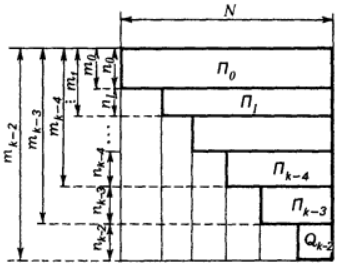
\includegraphics[width=\linewidth]{Image_3.png}
  \textbf{Рис. 8.}\\*
П$_1,$\hillП$_2,$\hfillП$_3, ...$\hfillВ\hfillкаждом\hfillпрямоуголь-\\*
нике\hfillП$_i$\hfillровно\hfill$n_i$\hfillстрок,\hfillв\hfillкаждой\hfillиз\hfillко-\\*
торых\hfillзакрашено\hfillпо\hfillкрайне\hfillмере\hfill$n_1$\\*
клеток,\hfillтак\hfillчто\hfillв\hfill$Q_0$\hfillво\hfillвсяком\hfillслучае\\*
закрашено\hfill$n_0^2 + n_1^2 + ... + n_{k-3}^2$клеток.\\*
Введем\hfillобозначения:\hfill$m_0 = n_0, m_1 =$\\*
$= n_0 + n_1, m_2 = n_0 + n_1 + n_2, ...$\hfill(см.\\*
рис. 8).\hfillРассмотрим\hfillбилет\hfillс\hfillномером\\*
$|0m_0m_1 ... m_{k-3}xy|$,\hfillгде\hfill x\hfillи\hfill y\hfill-\\*
некие\hfillдве\hfill"цифры",\hfillне\hfillменьше, \hfillчем\\*
$m_{k-3}$\hfill(то\hfillесть\hfillящик\hfillс\hfillномером\hfill$xy$\\*
"расположен"\hfillв\hfill$Q_{k-2}$).\hfillЛегко\hfillвидеть,\\*
что\hfillэтот\hfillбилет\hfillможно\hfillположить\hfillтолько\\*
в\hfillящик\hfillс\hfillномером\hfill$xy$.\hfillПоскольку\hfill$x$\hfillи\\*
\endminipage
\vfill
\columnbreak
\minipage{0.5\textwidth}
\begin{tabular}{|l|}
\hline
\\
\fontsize{14pt}{}\textbf{Задачи наших читателей}\\
\\
\hspace*{13mm}1. Доказать , что\hfill\\*
\hspace*{13mm}a) $  S_n = \frac{1}{2^2} + \frac{1}{3^2} +  \cdots$\hfill\\
\\
\hspace*{33mm}$\cdots + \frac{1}{n^2} < \frac{2}{3};$\hfill\\
\hspace*{13mm}б) $  P_n = \frac{1}{2} \cdot \frac{3}{4} \cdot \frac{5}{6}\times $\hfill\\
\\
\hspace*{23mm}$\times \cdots \frac{2n - 1}{2n}< \frac{1}{\sqrt{4n+1}}.$\hfill\\
\hspace*{33mm}\fontsize{12pt}{}Г. Пискарев\hfill\\
\hspace*{22mm}\fontsize{10pt}{}(Ярославская обл.)\hfill\\
\hspace*{13mm}2. Пусть в треугольнике\hfill\\*
\hspace{9mm}$ABC$\hspace{4mm}сторона\hspace{4mm}$AC$\hspace{2mm}---\hspace{2mm}са-\hfill\\
\hspace{9mm}мая\hspace{4mm}длинная\hspace{4mm}или\hspace{3mm}самая\hfill\\
\hspace{9mm}короткая.\hspace{4mm}Доказать,\hspace{4mm}что\hfill\\
\hspace{9mm}тогда\hspace{1mm}найдется\hspace{1mm}действитель-\hfill\\
\hspace{9mm}ное\hspace{2mm}число\hspace{2mm}$x$\hspace{2mm}такое,\hspace{2mm}что\hfill\\
\hspace{12mm}$|AB|^x = |BC|^x + |AC|^x$\\
\hspace{35mm}О. Лемещев\hfill\\
\hspace{40mm}(г. Омск)\hfill\\
\hspace*{13mm}3.\hspace{3mm}Существует\hspace{3mm}ли\hspace{2mm}нату-\hfill\\*
\hspace{9mm}ральное\hspace{1mm}число,\hspace{1mm}квадрат\hspace{1mm}кото-\hfill\\*
\hspace{9mm}рого\hspace{1mm}равен\hspace{1mm}сумме\hspace{2mm}квадратов\hfill\\*
\hspace{9mm}$1000$\hspace{2mm}последовательных\hspace{3mm}на-\hfill\\*
\hspace{9mm}туральных\hspace{2mm}чисел?\hfill\\*

\end{tabular}
\endminipage
\end{multicols}
\end{document}
